\newpage

\section{Návrh}

Na základe analýzy problémovej oblasti a existujúcich riešení sme sa rozhodli najprv použiť konvolučnú neurónovú sieť (jej popis a architektúra v kapitole \ref{nn_popis}), čo sa pretavilo aj do prvotných experimentov (kapitola \ref{first_experiments}) vykonávaných v rámci predmetu Počítačové videnie\footnote{http://vgg.fiit.stuba.sk/teaching/computer-vision/}.

\subsection{Návrh neurónovej siete}
\label{nn_popis}

Celá architektúra je načrtnutá na schéme na obrázku \ref{my_tensorboard_cnn} vytvorenej pomocou nástroja  TensorBoard\footnote{https://www.tensorflow.org/get\_started/summaries\_and\_tensorboard/}.

Jedná sa o jednoduchú sieť so vstupnou konvolučnou vrstvou pre spracovanie obrázkov. Táto vrstva obsahuje konvolučný filter (veľkosť \textit{5x5}) s aktivačnou funkciou sigmoid. Výstup z nej ďalej pokračuje do vrstvy združovania, kde sa použije operácia MAX s filtrom o veľkosti \textit{2x2} a krokom tiež s veľkosťou \textit{2}. Po nich nasleduje vrstva normalizácie, kde je celý výstup zlúčený do jednej širokej vrstvy. Za ňou sa nachádza plne prepojená vrstva (z angl. fully-connected layer) s aktivačnou funkciou sigmoid a vrstva výpadku (z angl. dropout layer\cite{dropout}), ktorej hodnota (v rozmedzí od 0 do 1) určuje, aké percentuálne množstvo neurónov aj s prepojeniami bude dočasne skrytých. Táto možnosť umožňuje počas učenia sa predchádzať pretrénovaniu. Za vrstvou výpadku už nasleduje iba výstupná vrstva a jej transformácia na 2D maticu, obrázok predstavujúci mapu výraznosti, ktorú chceme dostať.

Aktivačná funkcia sigmoid je použitá najmä preto, že mapa výraznosti je prakticky pravdepodobnostné rozdelenie, t. j. sieť sa snaží predikovať pravdepodobnosti výraznosti každého pixelu. Ako algoritmus učenia sme zvolili štandardný algoritmus spätného šírenia chyby (z angl. backpropagation) s trochu extravagatným FTRL optimizérom.

\begin{figure}[H]
	\begin{center}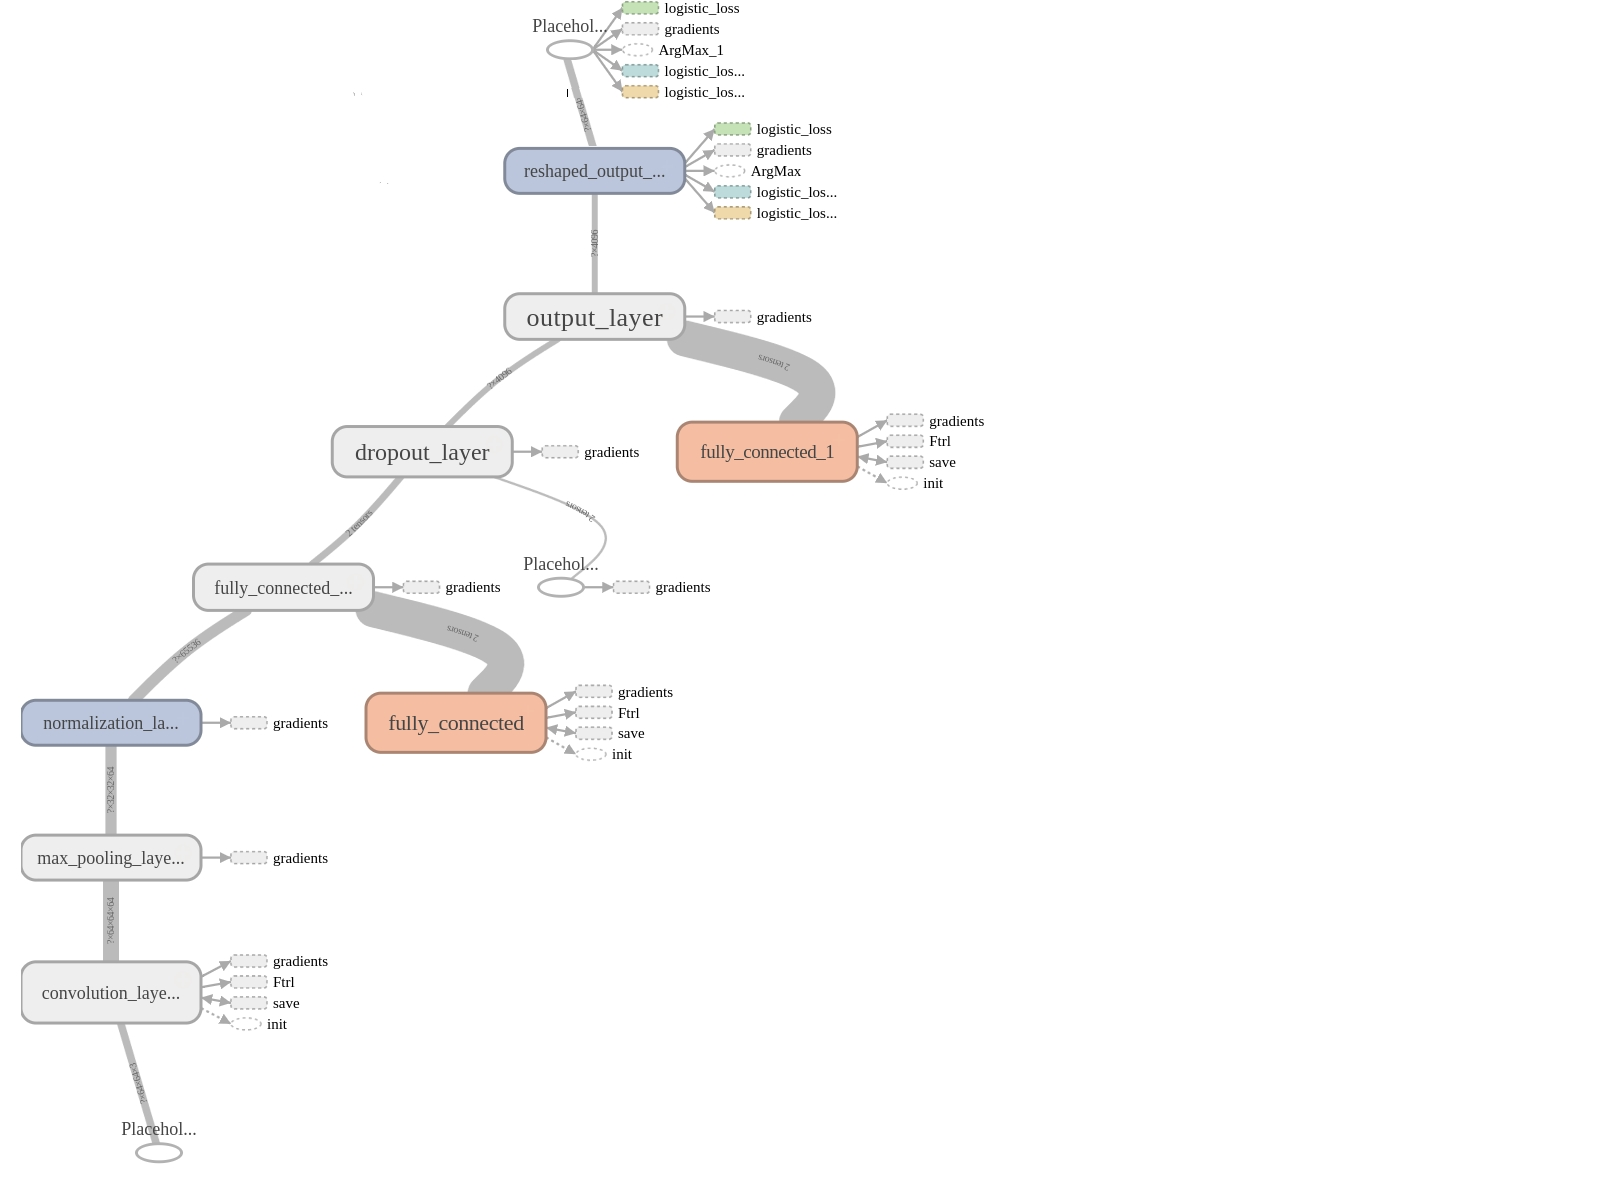
\includegraphics[scale=0.4]{graph-run.jpg}
		\caption[Návrh architektúry neurónovej siete]{
			Diagram reprezentujúci architektúru neurónovej siete, zdola vstupná konvolučná vrstva nasledovaná ostatnými vrstvami siete až po výstupnú, spolu s transformáciou na 2D maticu reprezentujúcu predikovanú mapu výraznosti pre vstupný obrázok
		}\label{my_tensorboard_cnn}
	\end{center}
\end{figure}
\iffalse
Na konvolučnej vrstve sa použije konvolučný filter o veľkosti 5x5, ktorým sa prejde vstupný obrázok. Výstupom z nej budú mapy (obrázky) po aplikovaní filtra. Tieto dáta budú spracovávané vo vrstve združovania s použitím operácie MAX, okna (filtra) s veľkosťou 2x2 a posunom s veľkosťou 2. Výstup všetkých filtrov je zlúčený do jednej širokej vrstvy a to normalizačnej. Z nej nasledujú prepojenia do plne prepojenej vrstvy, za ktorou nasleduje vrstva výpadku\cite{dropout}. Tá prakticky obsahuje hodnotu (od 0 do 1) určujúcu koľko neurónov bude dočasne „odstránených“ z modelu spolu so všetkými spojeniami, ako vstupnými tak aj výstupnými. To by malo zabrániť pretrénovaniu siete. Za vrstvou výpadku nasleduje už len výstupná vrstva, ktorá je nakoniec ešte aj transformovaná do 2D matice reprezentujúcej predikovanú mapu výraznosti. 

Aktivačná funkcia sigmoid bude použitá iba na prvej konvolučnej vrstve a na plne prepojenej vrstve. K trénovaniu sa použije FTRL optimizér spolu s náhodným generátorom dát, ktorý bude z datasetu určenému pre fázu trénovania náhodne vyberať dáta na učenie. Tým sa zabezpečí simulácia náhodnosti vstupných dát a teda sa sieť bude schopná lepšie učiť. 
\fi 

\subsection{Prvotné experimenty}
\label{first_experiments}

\subsubsection{Dataset}
\label{dataset}


\iffalse
\begin{equation}
content...
\end{equation}
\fi